\documentclass[11pt]{article}
\usepackage[textwidth=18.0cm, textheight=23.0cm, top=2.0cm]{geometry}
\usepackage{pst-all}
\usepackage{amssymb}
\usepackage{tikz}
\usepackage{underscore}\begin{document}
\pagestyle{empty}


ClassName: \underline{\textbf{Class_02.2bp-7}}
\par
BinSize: \underline{\textbf{30 × 30}}
\par
ReduceSize: \underline{\textbf{30 × 30}}
\par
TypeNum: \underline{\textbf{19}}
\par
Num: \underline{\textbf{20}}
\par
OutS: \underline{\textbf{900}}
\par
InS: \underline{\textbf{507}}
\par
Rate: \underline{\textbf{0.563}}
\par
UB: \underline{\textbf{1}}
\par
LB0: \underline{\textbf{1}}
\par
LB: \underline{\textbf{1}}
\par
LBWithCut: \underline{\textbf{1}}
\par
NodeCut: \underline{\textbf{0}}
\par
ExtendedNodeCnt: \underline{\textbf{1}}
\par
GenNodeCnt: \underline{\textbf{1}}
\par
PrimalNode: \underline{\textbf{0}}
\par
ColumnCount: \underline{\textbf{1}}
\par
TotalCutCount: \underline{\textbf{0}}
\par
RootCutCount: \underline{\textbf{0}}
\par
LPSolverCnt: \underline{\textbf{1}}
\par
PricingSolverCnt: \underline{\textbf{0}}
\par
BranchAndBoundNum: \underline{\textbf{1}}
\par
isOpt: \underline{\textbf{true}}
\par
TimeOnPrimal: \underline{\textbf{0.000 s}}
\par
TimeOnPricing: \underline{\textbf{0.000 s}}
\par
TimeOnRmp: \underline{\textbf{0.078 s}}
\par
TotalTime: \underline{\textbf{0.156 s}}
\par
\newpage


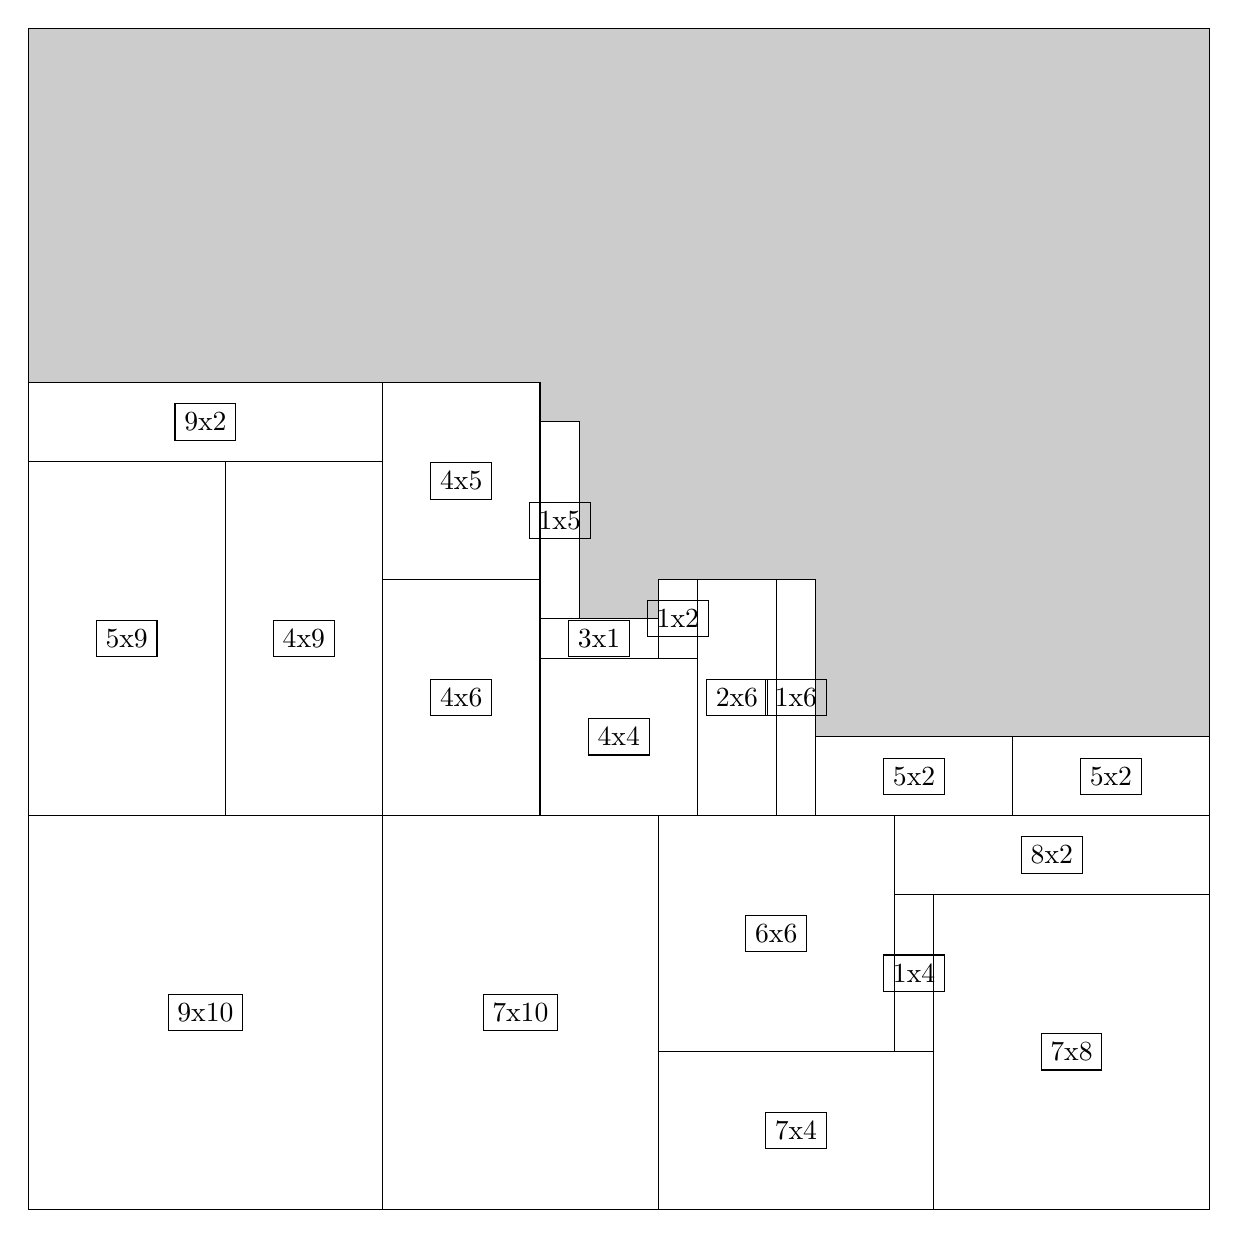
\begin{tikzpicture}[shorten >=1pt,scale=1.0,every node/.style={scale=1.0},->]
\tikzstyle{vertex}=[circle,fill=black!25,minimum size=14pt,inner sep=0pt]
\filldraw[fill=gray!40!white, draw=black] (0,0) rectangle (15.0,15.0);
\foreach \name/\x/\y/\w/\h in {9x10/0.0/0.0/4.5/5.0,7x4/8.0/0.0/3.5/2.0,7x8/11.5/0.0/3.5/4.0,5x9/0.0/5.0/2.5/4.5,6x6/8.0/2.0/3.0/3.0,4x9/2.5/5.0/2.0/4.5,7x10/4.5/0.0/3.5/5.0,4x6/4.5/5.0/2.0/3.0,4x5/4.5/8.0/2.0/2.5,9x2/0.0/9.5/4.5/1.0,8x2/11.0/4.0/4.0/1.0,4x4/6.5/5.0/2.0/2.0,2x6/8.5/5.0/1.0/3.0,5x2/10.0/5.0/2.5/1.0,5x2/12.5/5.0/2.5/1.0,1x6/9.5/5.0/0.5/3.0,1x5/6.5/7.5/0.5/2.5,1x4/11.0/2.0/0.5/2.0,3x1/6.5/7.0/1.5/0.5,1x2/8.0/7.0/0.5/1.0}
\filldraw[fill=white!40!white, draw=black] (\x,\y) rectangle node[draw] (\name) {\name} ++(\w,\h);
\end{tikzpicture}


w =9 , h =10 , x =0 , y =0 , v =90
\par
w =7 , h =4 , x =16 , y =0 , v =28
\par
w =7 , h =8 , x =23 , y =0 , v =56
\par
w =5 , h =9 , x =0 , y =10 , v =45
\par
w =6 , h =6 , x =16 , y =4 , v =36
\par
w =4 , h =9 , x =5 , y =10 , v =36
\par
w =7 , h =10 , x =9 , y =0 , v =70
\par
w =4 , h =6 , x =9 , y =10 , v =24
\par
w =4 , h =5 , x =9 , y =16 , v =20
\par
w =9 , h =2 , x =0 , y =19 , v =18
\par
w =8 , h =2 , x =22 , y =8 , v =16
\par
w =4 , h =4 , x =13 , y =10 , v =16
\par
w =2 , h =6 , x =17 , y =10 , v =12
\par
w =5 , h =2 , x =20 , y =10 , v =10
\par
w =5 , h =2 , x =25 , y =10 , v =10
\par
w =1 , h =6 , x =19 , y =10 , v =6
\par
w =1 , h =5 , x =13 , y =15 , v =5
\par
w =1 , h =4 , x =22 , y =4 , v =4
\par
w =3 , h =1 , x =13 , y =14 , v =3
\par
w =1 , h =2 , x =16 , y =14 , v =2
\par
\newpage


\end{document}